% \documentclass{report}
% 
% \usepackage{fancyhdr}
\usepackage{fourier-orns}
\usepackage{hyperref}%% To refrence links / jumps
\usepackage{chngcntr} %% For some extra counters numberings
\usepackage[a4paper, right = 0.5in, left = 0.5in,top = 1in , bottom = 1in]{geometry}
\usepackage{etoolbox} %% Provides like a language for advanced customization
\usepackage{datetime} %% For dates of course
\usepackage{lastpage} %% provides pages numbers
\usepackage[sc]{titlesec} %% modify titles
\usepackage{enumerate}
\usepackage{cancel}
\usepackage{tikzsymbols}
\usepackage[dvipsnames]{xcolor}
\usepackage{import}
\usepackage{pdfpages} %% include other pdfs
\usepackage{transparent} %% Transparency
\usepackage{xcolor}  %% Colors
\usepackage[many]{tcolorbox}
\usepackage[framemethod=TikZ]{mdframed}
\usepackage{amsmath,amsfonts,amsthm,amssymb,mathtools}
\usepackage{tikz}
\usepackage{bookmark}
\usepackage{graphicx}
\usepackage{mathpazo}

\usepackage{fontawesome5}

\linespread{1.5}


\titleformat{\chapter}[display]   
{\fontfamily{ppl}\selectfont\huge\color{YellowOrange!80!orange}} % Font style and size 
{\raggedleft\color{purple}\fontsize{70}{0pt}\selectfont\thechapter}   
{-1.5cm}    			                          % Space between the chapter number and title
{
	\begin{tikzpicture}[overlay]
		\node[anchor = west,yshift = 0.2cm,xshift = -1cm] {\fontsize{90}{20} $\int_{}^{} $};
		\node[yshift = 4cm, xshift = 17cm]   {\includegraphics[width = 4cm]{preview0}};
	\end{tikzpicture}
\hspace{1cm}\Huge\raggedright\MakeUppercase}

\titleformat{\section}[block]
{
\fontfamily{ppl}\selectfont\huge\color{YellowOrange!80!orange}
}
{
\color{purple}\fontsize{20}{0pt}\selectfont\thesection 
}
{0cm}
{
	\begin{tikzpicture}[overlay]
		\node[anchor = west,yshift = 0.2cm,xshift = -0.4cm, circle = 1pt] {};
	\end{tikzpicture}
}

\titlespacing*{\section}{0pt}{0.7cm}{1.5cm}


\newcommand{\divider}
{
	\begin{center}
	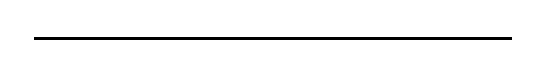
\begin{tikzpicture}
		\draw[thick, black] (0.25*\textwidth, 0) -- (0.75*\textwidth, 0);
		\node[rotate = 360 - 90, xshift = -0.6pt, yshift = 1pt] at (0.25*\textwidth,0){\decotwo};
		\node[rotate = 90, xshift = -0.6pt, yshift = 1pt] at (0.75*\textwidth,0){\decotwo};
	\end{tikzpicture}
	\end{center}
}

\pagestyle{fancy}

\newcommand{\lecday}[1][]
{
    \def\datee{#1}
    \fancyhead[L]{\datee}
}



\newcommand{\signature}
{
	\begin{tikzpicture}[remember picture,overlay]
		\node[fill = YellowOrange!20!white] at ([yshift = 1cm, xshift = -3cm]current page.south east) {\fontsize{10pt}{0pt}{\itshape Kara.$\mathcal{A}$}};
	\end{tikzpicture}
}

\AddToHook{shipout/background}{
  \begin{tikzpicture}[remember picture, overlay]
	  \node[] at ([yshift = 1.5cm,xshift = \textwidth /2 + 0.9cm]current page.south west) {\includegraphics[width = 0.5cm]{preview3}};
	  \node[] at ([yshift = 1.5cm,xshift = - \textwidth /2 - 0.9cm]current page.south east) {\includegraphics[width = 0.5cm]{preview4}};
  \end{tikzpicture}
}



\newtcolorbox[auto counter, number within = section]{remark}[1][]
{
       		title = Remark #1,
		enhanced,
		boxrule = 0pt,
		colback = white,
		breakable,
		arc = 4pt,
		colbacktitle = cyan,
		colback = cyan!5!white,
		segmentation style =
		{
			solid,cyan,thick,
		},
		attach boxed title to top left =
		{
			xshift = 0cm,
		},
		boxed title style =
		{
			boxrule = 0pt,
			sharp corners,
			drop fuzzy shadow = {cyan},
		},
		drop fuzzy shadow = {cyan!80!black},
}

\newtcolorbox[auto counter, number within = section]{theorem}[1][]
{                                      
		title = Theorem \thetcbcounter : #1,
		enhanced, 
		boxrule = 0pt,
		colback = white,
		breakable,
		arc = 4pt,
		colbacktitle = purple,
		colback = purple!5!white,
		segmentation style = 
		{
			solid, purple,thick,
		},
		attach boxed title to top left = 
		{
			xshift = 0cm, 
		},
		boxed title style = 
		{
			boxrule = 0pt,
			sharp corners,
			drop fuzzy shadow = {purple},
		},
		drop fuzzy shadow = {purple!80!black},
}

\newtcolorbox[auto counter, number within = section]{definition}[1][]
{                                      
		title = Definition \thetcbcounter : #1,
		enhanced, 
		boxrule = 0pt,
		colback = white,
		arc = 4pt,
		breakable,
		colbacktitle = YellowOrange!80!black,
		segmentation style = 
		{
			solid, YellowOrange,thick,
		},
		attach boxed title to top left = 
		{
			xshift = 0cm, 
		},
		colback = YellowOrange!5!white,
		boxed title style = 
		{
			boxrule = 0pt,
			sharp corners,
			drop fuzzy shadow = {YellowOrange!80!orange},
		},
		drop fuzzy shadow = {YellowOrange!80!black},
}

\newtcolorbox[auto counter, number within = section]{corollary}[1][]
{                                      
		title = corollary \thetcbcounter : #1,
		enhanced, 
		boxrule = 0pt,
		colback = white,
		arc = 4pt,
		breakable,
		colbacktitle = YellowOrange!80!black,
		segmentation style = 
		{
			solid, YellowOrange,thick,
		},
		attach boxed title to top left = 
		{
			xshift = 0cm, 
		},
		colback = YellowOrange!5!white,
		boxed title style = 
		{
			boxrule = 0pt,
			sharp corners,
			drop fuzzy shadow = {YellowOrange!80!orange},
		},
		drop fuzzy shadow = {YellowOrange!80!black},
}


\newtcolorbox{example}[1][]
{                                      
		title = Example,
		enhanced, 
		boxrule = 0pt,
		colback = white,
		arc = 4pt,
		segmentation style = 
		{
			solid, SpringGreen,thick,
		},
		breakable,
		colback = SpringGreen!5!white,
		colbacktitle = SpringGreen!80!black,
		attach boxed title to top left = 
		{
			xshift = 0cm, 
		},
		boxed title style = 
		{
			boxrule = 0pt,
			sharp corners,
			drop fuzzy shadow = {SpringGreen!80!orange},
		},
		drop fuzzy shadow = {SpringGreen!80!black},
}


\newcommand{\integral}[4]{\int\limits_{#1}^{#2} #4 d#3}
\newcommand{\limit}[3]{\lim\limits_{#1 \rightarrow #2} #3}
\newcommand{\strone}[2]{\left[ \begin{gathered}#1\\ #2\end{gathered} \right] }
\newcommand{\strtwo}[2]{\left\{ \begin{gathered}#1\\ #2\end{gathered} \right\} }
\newcommand{\strthree}[2]{\left\lfloor \begin{gathered}#1\\ #2\end{gathered} \right\rfloor }


\newcommand{\startbf}[1]{\text{\bfseries{#1}}}
\newcommand{\sett}[1]{\left\{ #1 \right\}}
\newcommand{\thesis}[1]{\left( #1 \right)}
\newcommand{\brkt}[1]{\left[ #1 \right]}
\newcommand{\floor}[1]{\left\lfloor #1 \right\rfloor}


\DeclareMathOperator{\img}{im} % Image
\DeclareMathOperator{\Img}{Im} % Image
\DeclareMathOperator{\coker}{coker} % Cokernel
\DeclareMathOperator{\Coker}{Coker} % Cokernel
\DeclareMathOperator{\Ker}{Ker} % Kernel
\DeclareMathOperator{\rank}{rank}
\DeclareMathOperator{\Spec}{Spec} % spectrum
\DeclareMathOperator{\Tr}{Tr} % trace
\DeclareMathOperator{\pr}{pr} % projection
\DeclareMathOperator{\ext}{ext} % extension
\DeclareMathOperator{\pred}{pred} % predecessor
\DeclareMathOperator{\dom}{dom} % domain
\DeclareMathOperator{\ran}{ran} % range
\DeclareMathOperator{\Hom}{Hom} % homomorphism
\DeclareMathOperator{\Mor}{Mor} % morphisms
\DeclareMathOperator{\End}{End} % endomorphism


\newcommand{\lm}{\ensuremath{\lambda}}
\newcommand{\eps}{\ensuremath{\epsilon}}
\newcommand{\veps}{\ensuremath{\varepsilon}}
\newcommand{\al}{\ensuremath{\alpha}}
\newcommand{\bb}{\ensuremath{\beta}}
\newcommand{\cc}{\ensuremath{\gamma}}
\newcommand{\dd}{\ensuremath{\delta}}
\newcommand{\DD}{\ensuremath{\Delta}}
\newcommand{\ff}{\ensuremath{\phi}}
\newcommand{\FF}{\ensuremath{\varphi}}

\newcommand{\RR}{\mathbb{R}}
\newcommand{\RO}{\mathcal{R}}
\newcommand{\EE}{\mathbb{E}}
\newcommand{\CC}{\mathbb{C}}
\newcommand{\RW}{\mathbb{R}^2}
\newcommand{\RT}{\mathbb{R}^3}
\newcommand{\RN}{\mathbb{R}^n}
\newcommand{\DS}{\mathcal{D}}

\newcommand{\KK}{\mathbb{K}}
\newcommand{\KW}{\mathbb{K}^2}
\newcommand{\KT}{\mathbb{K}^3}
\newcommand{\KN}{\mathbb{K}^n}

\newcommand{\NN}{\mathbb{N}}

\newcommand{\PS}{\mathcal{P}}
\newcommand{\AS}{\mathcal{E}}
\newcommand{\FS}{\mathcal{F}}
\newcommand{\LS}{\mathcal{L}}
\newcommand{\MS}{\mathcal{M}}

















% 
\lecday[2025-04-24]

% \begin{document}

\it Corollary : \normalfont 
Let $E $ be a Banach space and $F $ an $G $ be two arbitrary N.V.S. 
let also $ h : E \times F  \longrightarrow G $ be a bilinear mapping that is separately 
continuous, that is $h $ satisfies the following properties, 
\begin{enumerate}[(1)]
\item  for all $y \in  F $, the linear mapping 
	\[
	\begin{array}{cccc}
	      h(.,y)  : &  E  & \longrightarrow & G \\
	
	           &  x  & \longmapsto     & h(x,y)  \\ 
	\end{array}
	\]
	is continuous
\item for all $x \in  E $, the linear mapping 
	\[
	\begin{array}{cccc}
	      h(x,.)  : &    F& \longrightarrow &  G\\
	
	           &y    & \longmapsto     &  h(x,y) \\
	\end{array}
	\]
	is continuous  
\end{enumerate}
Then $h $ is \it continuous \normalfont
\begin{proof}
Define 
\[
A = \left\{ h(., y) : y \in  \overline{B_{F}}(0_{F},1)   \right\} \subset 
\mathcal{L} (E,G) 
\]
and for all $x \in E $, 
\begin{align*}
	A_{x} &:= 
\left\{ f(x) , f \in  A \right\} \\
&= \left\{ h(x,y) , y \in \overline{B_{F}}(0_{F},1)  \right\} \\
&= \left\{ h(x,.)(y), y \in \overline{B_{F}}(0_{F},1)   \right\}
\end{align*}
Giving $x \in E  $, since the linear mapping 
$h(x,.)  $  is continuous by hypothesis then the last
inequality shows that the subset $A_{x} $ of $G $ is bounded. Thus (by Banach
Steinhaus theorem), the subset $A$ of $\mathcal{L} (E,G)  $ is bounded (say
by a pointwise constant $M $). Hence, we have for all 
$x \in  \overline{B_{F}}(0_{E},1)  $ and $y \in \overline{B_{F}}(0_{F},1)$,
\begin{align*}
	\| h(x,y)  \| _{G} &= \| h(.,y)(x)   \| _{G} \\ 
			   & \leq 
			   \mid \mid \mid  
			   \underbrace{
			   h(.,y)
			   }_{ \in A} 
			   \mid \mid \mid _{ \mathcal{L} (E,G) } 
	\cdot \| x \| _{E}  \leq  M
\end{align*}
implying that $h $ is continuous, hence the corollary is proved.
\end{proof}
\divider
\chapter{Quotient vector normed spaces :}

Let $E $ be a N.V.S. and $H $ be a vector subspace of $E $. Recall that 
the quotient vector space of $E $ on $H $ is given by, 

\[
E_{ \backslash H}= 
\left\{ x + H, x \in  E \right\} 
\]
Consider the map 
\[
\begin{array}{cccc}
	\| . \| _{E _{ \backslash H}} : &  E_{ \backslash H}  & \longrightarrow & [0,\infty ) \\

           &    C & \longmapsto     &  \inf_{ x \in  C} \| x \| _{E}\\ 
\end{array}
\]
the map $\| . \| _{E _{ \backslash H}} $  defines a seminorm 
on $E _{ \backslash  H} $. In addition, $\| . \| _{E \backslash H} $  
becomes a norm on $E _{ \backslash H} $ if and only if $H$ 
is closed in $E$.
\begin{proof}
Let us show that the map $\|. \| _{E _{ \backslash H}} $
satisfies the three properties of 
a seminorm on the quotient vector space $E_{ \backslash H}$.
\begin{enumerate}
\item The zero vector of the quotient vector space $E _{ \backslash H} $  
	is $C(0_{E}) = 0_{E} + H = H  $, and we have, 
	\[
	\| H \| _{E _{ \backslash H}} = 
	\inf_{x \in  H}  \| x \| _{E} \leq     
	\| 0_{E} \|_{E} 
	\]
	Thus, $\| H \| _{E \backslash H} = 0 $, as required.
\item Let $\lm \in  \KK $   and $C \in  E_{ \backslash H} $, 
	since $\lm C = \left\{ \lm x, x \in  C \right\} $ then we have, 
	\begin{align*}
		\| \lm C_{E_{ \backslash H}} \|  &= 
		\inf_{x \in  C}  \| \lm x \| _{E} \\
						 &= 
			\inf_{x \in  C}  \left( 
				\left| \lm \right| 
				\| x \|_{E} 
			\right) \\
			 &= \left| \lm \right| 
			 \left( \inf_{x \in  C} 
				 \| x \|_{E} 
			  \right) = 
			  \left| \lm \right| 
			  \| C \|_{E_{ \backslash H}} 
	\end{align*}
	as required.
\item Let $C_1, C_2 \in  E_{ \backslash H} $   
	which we can write as 
	\[
	C_1 = x_1 + H \quad 
	C_2 = x_2 + H
	\]
	where $x_1, x_2 \in E $,
	\[
	\| C_1 + C_2 \|  _{E _{ \backslash H}} 
	\overset{?}{ \leq }  
	\| C_1 \| _{E _{ \backslash H}} + 
	\| C_2 \| _{E _{ \backslash H}}
	\]



	then $C_1 + C_2 = 
	x_1 + x_2 + H$, By the triangle inequality in $E $, we have
	for all $h_1, h_2 \in  H $, 
	\[
		(x_1 + h_1)  + (x_2 + h_2)   
		\leq \| x_1 + h \|  _{E } + 
		\| x_2 + h_2 \|  _{E}
	\] 
	taking in the two sides of this inequality the infimum where 
	$h_1, h_2 \in H $, we obtain since $(\left\{ h_1 + h_2, 
	h_1,h_2 \in H\right\} = H)$
	\begin{align*}
	\inf_{h \in H}  
	\| x_1 + x_2 + h \| _{E} & \leq 
	\inf_{h_1 \in  H}  
	\| x + h_1 \|  + \inf_{h_2 \in  E}  \| x + h_2 \| _{E} 
	\end{align*}
	That is 
	\[
		\| C_1 + C_2 \|  _{E _{ \backslash H}} 
		 \leq 
		\| C_1  \| _{E _{ \backslash H}} + 
		\| C_2 \| _{ E_{ \backslash H}}
	\]
	as required. Consequently, 
	$\| . \| _{E _{ \backslash H}} $  defines a seminorm 
	on $E \backslash H$. \\
	Next, denoting by $d $ the metric associated to the norm
	of $E $, we have for all $x \in  E $, 
	\begin{align*}
		\| x + H \|  _{E \backslash H} 
		&= \inf_{h \in  H}   
		\| x+h \| _{E} \\
		&= \inf_{h \in  H}  
		\| x - h \| _{E} \\
		&= \inf_{h \in H}  
		d(x,H)  \\
		&= d(x;H) 
	\end{align*}
	It follows according to the well-known results on metric spaces, 
	that for all $x \in  E $, 
	\begin{align*}
		\| x + H \| _{E \backslash H} = 0 & 
		\iff 
		d(x,H)  = 0  
	\\
						  & \iff 
			x \in  \overline{H}
	\end{align*}
	Therefore, $\| . \| _{E _{ \backslash H}} $  
	defines a norm on $E_{ \backslash H}$  if 
	and only if $\overline{H} = 0_{E \backslash H} = H $, that 
	is if and only if $H $ is closed in $E $, the proof is complete.
\end{enumerate}
\end{proof}
\begin{center}
	\textbf{Terminology : }
\end{center}
The map $ \| . \| _{E _{ \backslash H}} $  defined above is 
called the quotient seminorm of $E _{ \backslash H} $, if $H $ 
is closed in $E $, its called the quotient norm of $E _{ \backslash H} $.
\divider
\lefthand ~ \it NB : \normalfont whenever the quotient 
space $E _{ \backslash H} $  is mentioned (where $E $ is N.V.S. and $H $ is 
closed vector subspace of $E $ ) its completely assumed that 
$E \backslash H $  is equipped with the quotient norm 
$\| . \| _{E _{ \backslash H}} $  defined previously.
\divider
\begin{theorem}[]
Let $E $ be a N.V.S. and $H $ be a closed \it proper \normalfont subspace of 
$E$.  then the quotient map 
\[
\begin{array}{cccc}
      \Pi  : &  E  & \longrightarrow & E_{ \backslash H} \\

             x&    & \longmapsto     &  x + H\\ 
\end{array}
\]
is continuous, and satisfies $ \mid \mid \mid  \pi  \mid \mid \mid = 1 $ 
\end{theorem}
\begin{proof}
Recall that $\pi  $ is linear. Next, for all $x \in  E $, we have, 
\begin{align*}
\| \pi  (x)  \|  _{E \backslash H}
= 
\| x + H \| _{E _{ \backslash H}}  
&:= 
\inf_{h \in H}  \| x + h \| _{E} 
\\
& \leq 
\| x + 0_{E} \| _{E} = \| x \| _{E}
\end{align*}
implying that $\pi$ is continuous and that 
\[
\mid \mid \mid  \pi  \mid \mid \mid  \leq 1
\]
Now, let us show that  
\[
\mid \mid \mid  \pi  \mid \mid \mid  \geq 1
\]
To do so, fix $a \in E \backslash H $, thus
$\pi (a)  \neq  H = 0_{E _{ \backslash H}}$,
implying that $\| \pi (a)  \| _{E _{ \backslash H}} > 0$, 
by definition of $\| \pi (a)  \| _{E _{ \backslash H}} $ 
and the characterization of the infimum of a 
subset of $\RR  $, 
\[
	\| \pi (a)  \|  _{E _{ \backslash H}} 
	= \inf_{x \in  \pi (a) }  
	\| x \| _{E} 
\]
for all $ \veps > 0 $, there exist 
$x_{E} \in \pi (a) $ such that, 
\begin{align*}
\| \pi (a)  \|  _{E _{ \backslash H}}   
&\leq 
\| x_{ \veps } \|  _{E} 
 \\
& \leq 
\| \pi (a)  \|  _{E _{ \backslash H}} + 
\veps 
\end{align*}
implying that, 
\[
\frac{\| \pi (x_{a})  \|_{E_{ \backslash H} }}{ \| x_{ \veps } \|_{E} } 
\geq 1 - \frac{me}{\| x_{ \veps } \| _{E}} 
\geq 
1 - \frac{\veps }{\| \pi (a)  \| _{E_{ \backslash H} }}
\]
Thus, 
\begin{align*}
\mid \mid \mid  \pi  \mid \mid \mid  = 
\sup_{x \in  E \backslash \left\{ 0_{E} \right\}}  
\frac{\| \pi (x)   \|_{ E_{ \backslash H} } }{ \| x \|_{E} } 
& \geq 
\frac{\| \pi (x_{ \veps })  \| _{E_{ \backslash H} }}{\| x_{\veps } \| _{E}} 
\\
& \geq 1 - \frac{ \veps }{\| \pi (a)  \| _{E_{ \backslash H} }}
\end{align*}
hence 
\[
\mid \mid \mid  \pi  \mid \mid \mid  \geq 1 - 
\frac{\veps }{\| \pi (a)  \| _{E_{ \backslash H} }}
\]
by taking $ \veps  \rightarrow  0^{+} $  
gives $\mid \mid \mid  \pi  \mid \mid \mid  \geq 1$, as required 
here $\mid \mid \mid  \pi  \mid \mid \mid =1 $, completing this proof.
\end{proof}
\begin{theorem}[]
Let $E $ be a Banach N.V.S. and $H $ be a closed vector subspace
of $E $, then $E_{ \backslash H} $  is Banach.
\end{theorem}
\begin{proof}
To show that $E \backslash H $  is Banach, we will prove that every
normally convergent series in $E_{ \backslash H}  $  
is convergent, Let 
$\sum_{n=1}^{\infty }C_{n}  $  be a normally convergent series in 
$E_{ \backslash H}  $, This means that the real series 
$\sum_{n=1}^{\infty } \| C_{n} \| _{E_{ \backslash H} } $  
is convergent, by the definition of $\| C_{n} \| _{E_{ \backslash H} } (=
\inf_{x \in C_{n}}  \| x \| _{E} )$, and the chracterzation of the 
infimum of a subset of $\RR  $, for all $n \in \NN$, there exist 
$x_{n} \in  C_{n} $  such that 
\[
\| x_{n} \|  _{E} 
\leq \| C_{n} \| _{E_{ \backslash H} } + 
\frac{1}{2^n }
\]
This implies that the real series 
\[
\sum_{n=1}^{\infty } \| x_{n} \| _{E}
\]
converges, namely the series  
$\sum_{n=1}^{\infty } x_{n} $  is normally convergent
in $E $, but since $E $ is Banach, it follows that the series
$\sum_{n=1}^{\infty } x_{n} $  is convergent in $E $. Finally,
since $\pi  $ is continuous (according to proposition $2 $), we conclude
that the series $\sum_{n=1}^{\infty } \pi (x_{n}) =
\sum_{n=1}^{\infty } C_{n}$ is convergent in $E \backslash H $, as required
therefore $E_{ \backslash H}  $  is Banach, completing the proof.
\end{proof}




\begin{center}
	\it The Hahn-Banach theorem \normalfont
\end{center}
\textbf{PreLiminaries : } 
\begin{theorem}[Zorn's Lemma]
	Let $X $ be partially ordered
	suppose that every \it chain \normalfont $\mathcal{C}$ in $X $, 
	(That is, every totally ordered subset of $X $), 
	has an upper bound in $X$. Then $X $ contains atleast one
	maximal element 
\end{theorem}
\divider
\it Note : \normalfont  $m $ is upper-bound
\[
\forall x \in A, x \leq m 
\]
\divider
\begin{example}
\begin{theorem}[]
	Every vector space has a basis. (Teacher provided a Skratch proof, we
	may prove it next time)
\end{theorem}
\end{example}
% \end{document}



%
%        E            F
%     +----+        +----+    
%     -    -        -    -    
%     +----+        +----+    
%                    -
%              G    -
%                  v
%           +------+
%           -      -
%           +------+
%




